\section{Negativ återkoppling}

\paragraph{Vad är negativ återkoppling?}
I denna kursen kommer vi att studera hur man kontrollerar ett system vid att låta avvikelsen mot det önskade värdet kontrollera regleringen av storheten.

\paragraph{Illustration i blockdiagram}
Ett enkelt negativt kontrollsystem illustrearas i figur \ref{fig:negative_feedback}.

\begin{figure}[!ht]
	\centering
	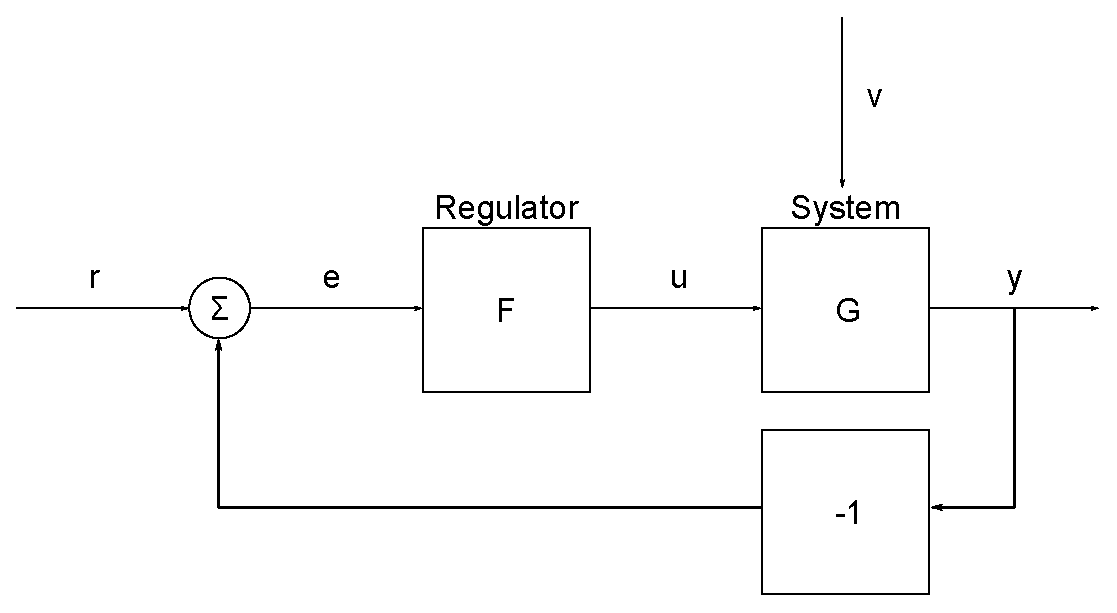
\includegraphics[width = \textwidth]{./Images/negative_feedback.eps}
	\caption{Schematisk illustration av ett enkelt negativt återkopplad system.}
	\label{fig:negative_feedback}
\end{figure}

\paragraph{Beskrivning av systemet}
Vi börjar beskrivningen av systemet med att inte betrakta störningar. I ena ändpunkten har vi
\begin{align*}
	Y = GU = GFE.
\end{align*}
Summationskomponenten till vänster ger oss
\begin{align*}
	E = R - Y,
\end{align*}
och därmed
\begin{align*}
	Y = GFR - GFY.
\end{align*}
Därmed kan vi skriva
\begin{align*}
	Y = \frac{GF}{1 + GF}R.
\end{align*}

\paragraph{Återkopplad överföringsfunktion}
För ett återkopplad system som kan skrivas som $Y = G_{\text{C}}R$ definieras $G_{\text{C}}$ som den återkopplade överföringsfunktionen. För systemet ovan har vi alltså
\begin{align*}
	G_{\text{C}} = \frac{GF}{1 + GF}R.
\end{align*}

\paragraph{Samband mellan reglerfel och referens}
Alternativt kan vi lösa systemet ovan för att få
\begin{align*}
	R - E = GFE,\ E = \frac{1}{1 + GF}R.
\end{align*}

\paragraph{Samband mellan referens och insignal}
Systemet ovan kan även lösas för att ge
\begin{align*}
	U = FR - FY = FR - GFU,\ U = \frac{F}{1  + GF}R.
\end{align*}

\paragraph{Slutna systems poler}
Vi ser att slutna system har poler där $1 + GF = 0$. Därmed bestäms systemets stabilitet av systemet och regulatorn.